\chapter{Nanotechnology and the Future of Computation, Storage and Perception}

\begin{center}
{\large\uppercase{Navakanta Bhat}}

\vskip -6pt

Professor and Chair, Centre for Nano Science and Engineering\\ Indian Institute of Science, Bangalore-560012
\end{center}
\vskip .5cm

\noindent\makebox[\textwidth]{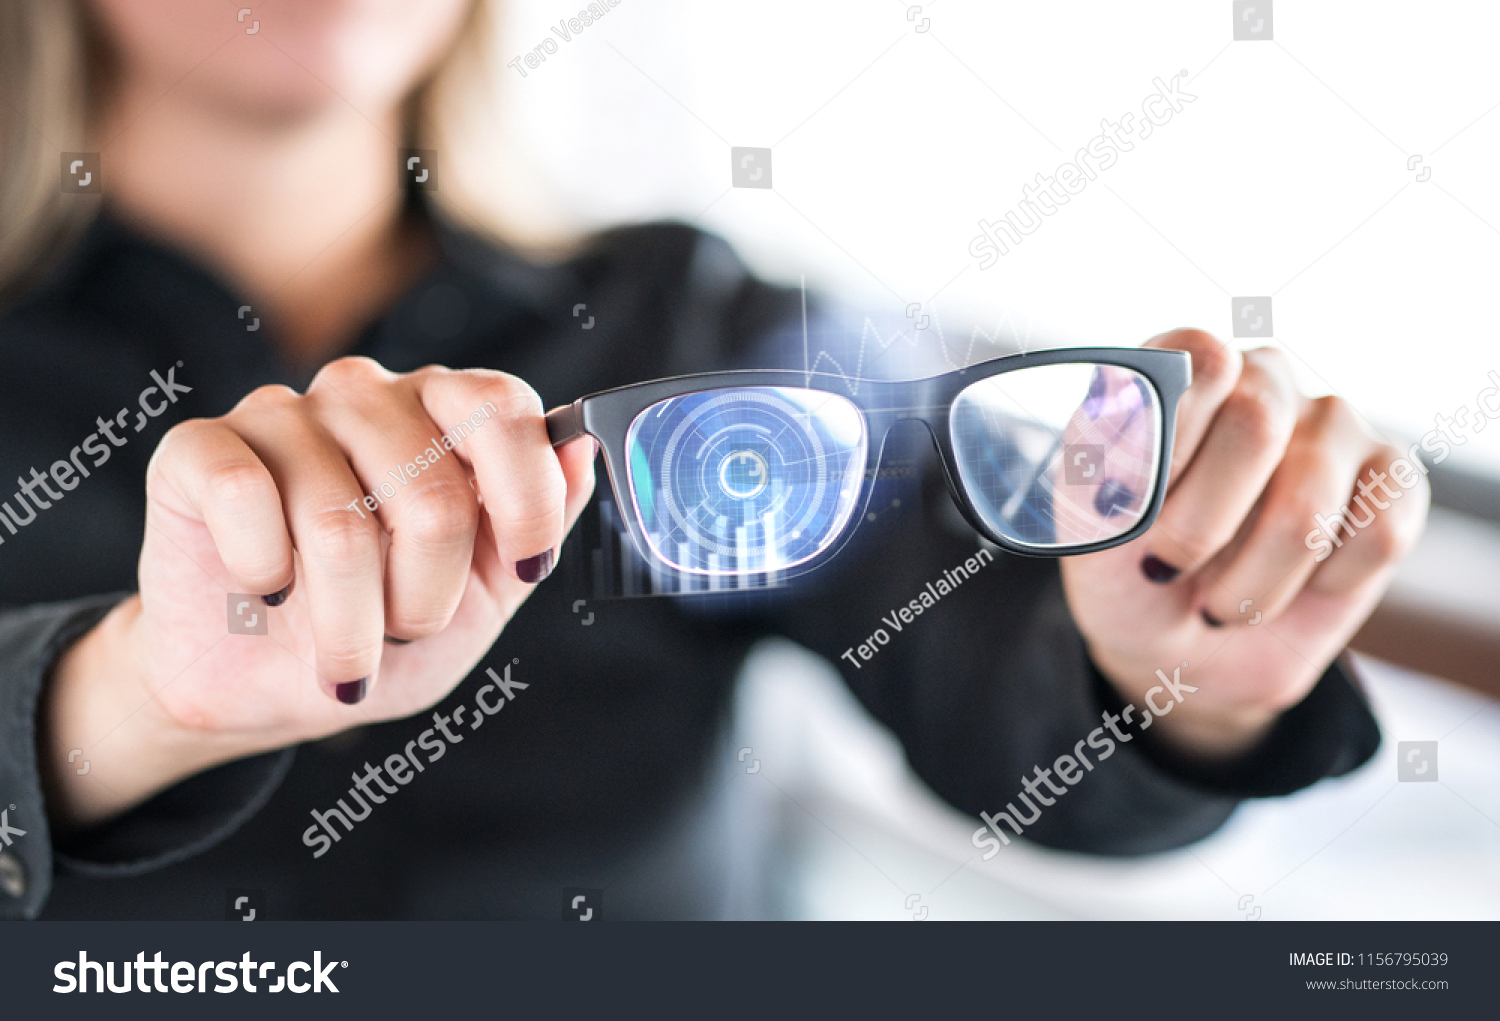
\includegraphics[width=1.05\paperwidth,height=15cm]{src/Figures/Nano.jpg}}

\newpage

\begin{multicols}{2}

\section{Historical Perspective and Current Status}

The continued miniaturization of devices in the nanoscale regime, and the capability to manipulate the matter at these dimensions is expected to revolutionize the future systems for computation, storage and perception in the next few decades. Nanotechnology is not just a natural evolution of the miniaturization trend from sub-100 micrometer scale to sub-100 nanometer scale. The emergence of quantum effects at nanoscale, with a significant departure from  the continuum approximation of physical, chemical and biological processes, brings in exciting new possibilities with nanotechnology. In the next few decades, we will go beyond the conventional charge based, digital Silicon CMOS technology, and incorporate several emerging technologies that exploit nanoscale phenomena, to realize extremely powerful machines for high performance computation with augmented perception, mimicking the human brain and sensory organs. 

Figure~\ref{chap1-fig1} depicts  the key milestones in the evolution of compute engines. The bulky and power hungry vacuum tubes used in one of the early digital computers, ENIAC, resulted in rudimentary computation capabilities with the computer weighing 30 tons and consuming 200 kW power. This was certainly not a scalable technology. The invention of semiconductor transistor in 1947 was an inflexion point in the history of miniaturization. This was followed by the invention of the first integrated circuit (IC), a decade later in 1958. However, most of the early ICs were only memory chips and the community was concerned as to what one would do with all those storage devices. Then, the first microprocessor IC invented in 1971,  changed the landscape completely. The Intel 4004, a 4 bit microprocessor was realized on 10 $\mu\mbox{m}$ PMOS technology, with a chip size of 12 $\text{mm}^2$ and power consumption of 1W. This was soon followed by migration to  NMOS technology (Intel 8080 in 1974) and CMOS technology (Intel 80386 in 1985).  As exemplified by the famous Moore’s law, the miniaturization trend has continued with CMOS technology scaling, resulting in a new generation of manufacturing technology introduced every 2 to 3 years. This technology scaling,  coupled with several innovations in system and circuit architectures, has fuelled the growth of more and more powerful compute engines over the years. For instance, in 2013, the CMOS technology went through another big change with the introduction of 3 dimensional (3D) FinFETs, departing from the conventional planar MOSFETs (Figure~\ref{chap1-fig2}). By this time, the CMOS technology was also enabled by innovations in nanomaterials technology such as strained Silicon-Germanium channel, $\mbox{HfO}_2$ high-k gate dielectric with atomically engineered interface. On the architectural front, the introduction of multi-core processors, brought in an unprecedented computing capabilities, even to the hand held devices.  
\begin{figure}[H]
\centering
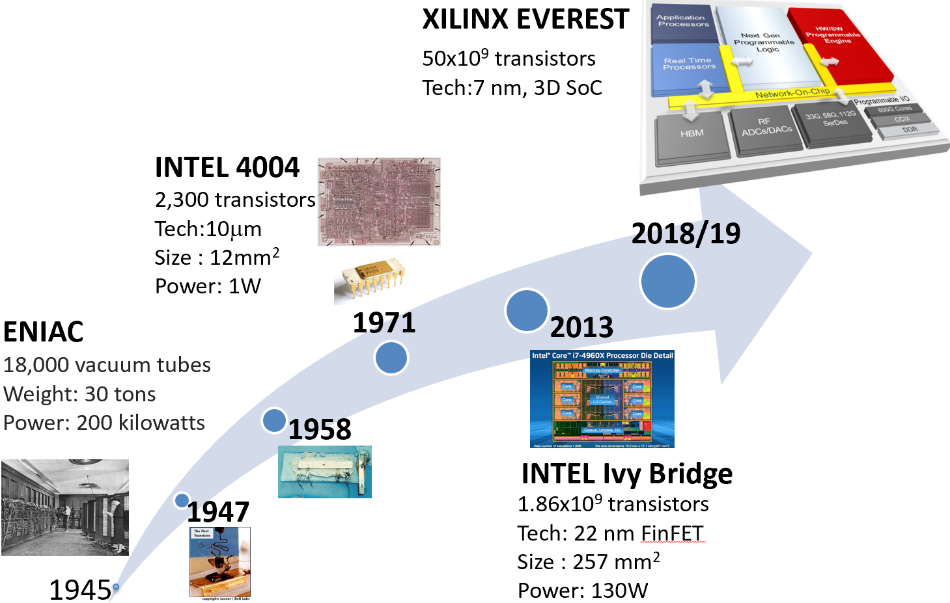
\includegraphics[scale=1.1]{src/Figures/chap1/chap1-fig01.jpg}
\caption{Evolution of computation chips [the illustrative images are from Intel and Xilinx]}\label{chap1-fig1}
\end{figure}

\begin{figure}[H]
\centering
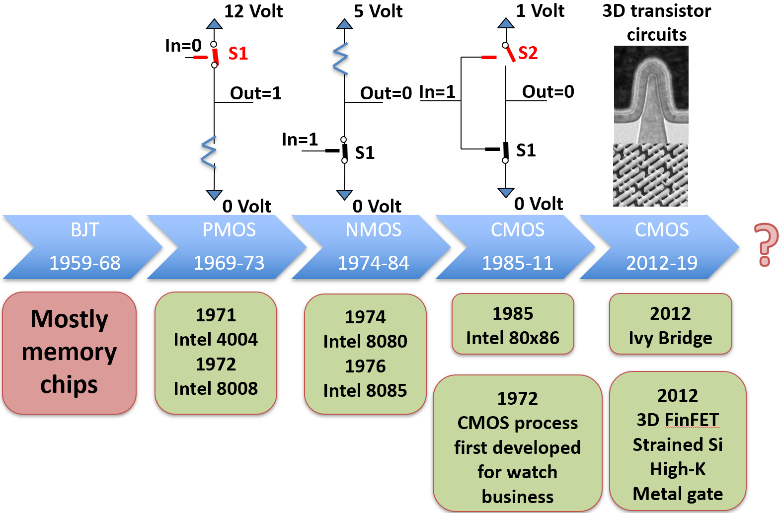
\includegraphics[scale=1.2]{src/Figures/chap1/chap1-fig02.jpg}
\caption{Evolution of transistor technology with an\break illustration of inverter implementation}\label{chap1-fig2}
\end{figure}

The Everest chip from  XILINX, on 7nm CMOS technology with 3D System on Chip fabric, packs 50 billion transistors on single chip, illustrating an amazing technological achievement. It should be recognized that in conjunction to miniaturization, the integration of  exponentially large number of transistors is primarily responsible for today’s high performance compute and storage chips. As shown in Figure~\ref{chap1-fig3}, over the last 5 decades, while the “feature size” of transistors has scaled down by  3 orders of magnitude $(10^{-3})$, the number of components on chip has been increased by 7 orders of magnitude $(10^7)$. In conjunction with migration from microtechnology to nanotechnology, we have also moved from Small Scale Integration (SSI) to Very Large Scale Integration (VLSI) or Giga Scale Integration (GSI).

\begin{figure}[H]
\centering
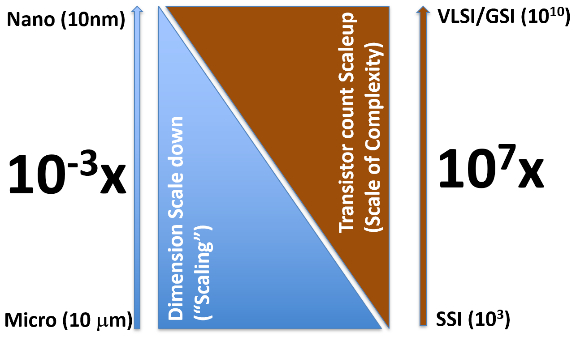
\includegraphics[scale=1.3]{src/Figures/chap1/chap1-fig03.jpg}
\caption{Transistor size scaling, coupled with exponential increase of transistor count}\label{chap1-fig3}
\end{figure}

In addition to the underlying nanoscale CMOS technology and ever evolving system and circuit architecture, the highly complex and powerful chips of today owe it to another key enabler, namely the Electronics Design Automation (EDA) using Computer Aided Design (CAD) tools. It is not hard to appreciate that the designing of giga scale integrated circuits would be impossible without sophisticated CAD tools. In late 70s, the handcrafting of the transistors on a chip, turned out to be unmanageable. This led to the emergence of hierarchical abstraction of various components of the chip at behavioural, structural, functional and physical level. The design concepts put forth by Mead and Convey, eventually led to commercial CAD tools to assist in the design of complex chips. Today there is an interesting symbiosis: the advanced CAD tools enabling advanced chips, which in turn enable advanced compute engines that are capable of supporting further advances in CAD tools. The CAD tools have matured so much that the design of a complex chip is akin to writing a software code, through hardware description languages such as Verilog and VHDL. Through the accurate modelling abstraction at different levels, it is possible to achieve first pass success, from specification to the fabrication of a chip, through logic synthesis and layout synthesis tools (Figure~\ref{chap1-fig4}). For any other emerging nanotechnology option to be  successful, it is extremely important to have similar CAD tools to manage complex designs. 
\end{multicols}

\begin{figure}[H]
\centering
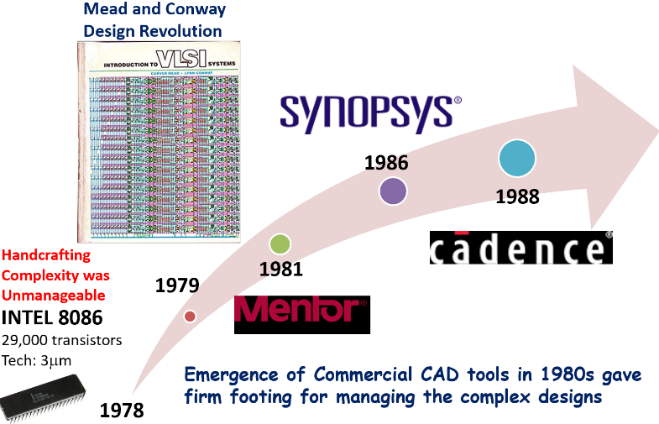
\includegraphics[scale=1.3]{src/Figures/chap1/chap1-fig04a.jpg}\qquad\qquad
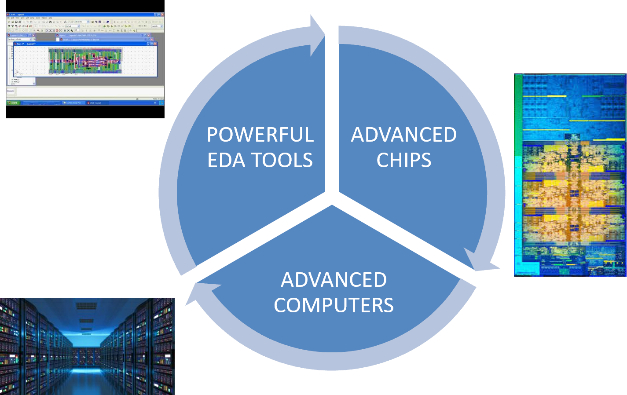
\includegraphics[scale=1.3]{src/Figures/chap1/chap1-fig04b.jpg}\\[35pt]
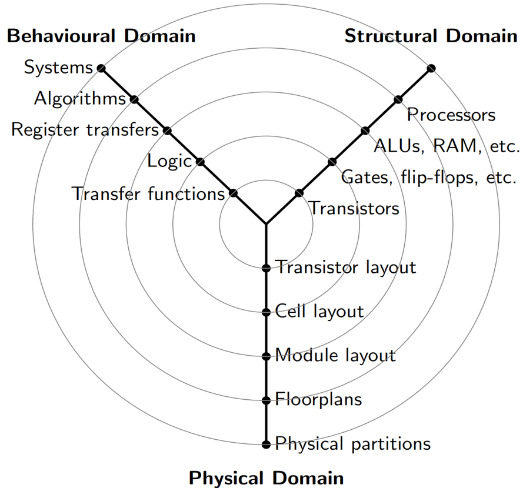
\includegraphics[scale=1.3]{src/Figures/chap1/chap1-fig04c.jpg}\qquad\qquad
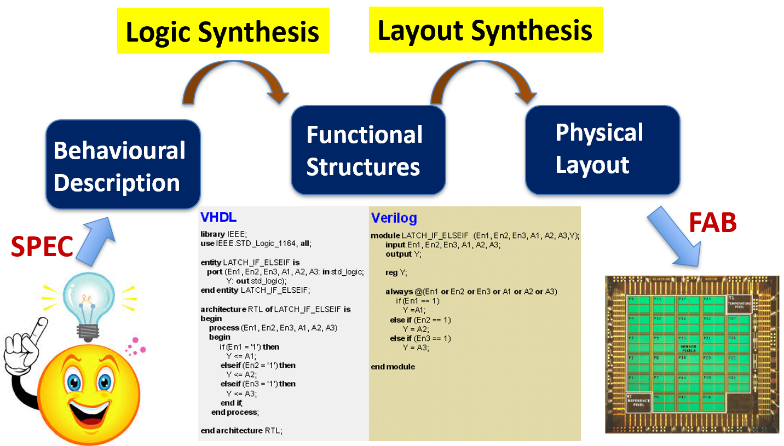
\includegraphics[scale=1.3]{src/Figures/chap1/chap1-fig04d.jpg}
\caption{The emergence of CAD tools for the design of complex chips, with a symbiotic positive feedback between EDA tools, advanced chips and high performance computers.  “Gajski-Kuhn Y chart” illustrating abstraction at behavioural, structural and physical domains. EDA tools enabling the “chip design compilers”}\label{chap1-fig4}
\end{figure}

\vfill\eject


\section{Future Directions} 
\begin{figure}[H]
\centering
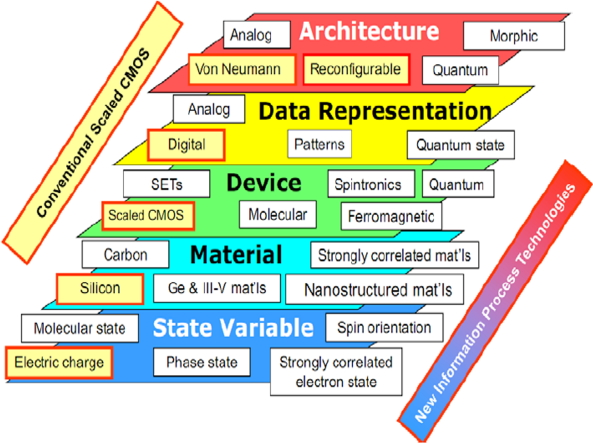
\includegraphics[scale=1.2]{src/Figures/chap1/chap1-fig05a.jpg}\qquad\qquad
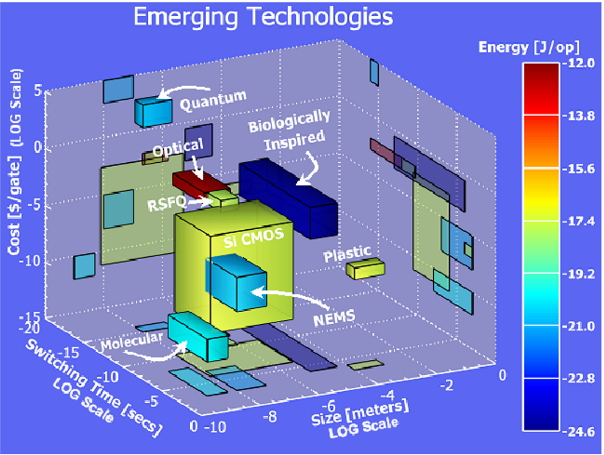
\includegraphics[scale=1.2]{src/Figures/chap1/chap1-fig05b.jpg}
\caption{The hierarchical view of compute and storage technologies and the representation of emerging technologies along multiple performance metrics (\url{http://www.itrs2.net/})}\label{chap1-fig5}
\end{figure}

\begin{multicols}{2}
With CMOS technology entering the sub-10nm regime, fundamental road blocks are appearing with respect to the underlying materials/process technology and device physics.  The big question haunting us quite often is “whether Moore’s law is hitting a red brick wall”? This conundrum can be solved only through some fundamental breakthroughs in nanotechnology in the future. In this context, the guidelines of International Technology Roadmap for Semiconductors (Figure~\ref{chap1-fig5}), are very instructive. 

The current compute and storage technologies use “electric charge” as \textit{state variable}, with “silicon” as the de-facto \textit{material,} “scaled CMOS” as the \textit{device} for “digital” \textit{data representaion} under “von Neumann” computation \textit{architecture.}  At each of these hierarchical levels, multiple other approaches are possible. For instance, the state variable could exploit “spin” of the electrons to build \textit{spintronic} devices. Alternately, the state variable could be “strongly correlated electronic state”, to build \textit{quantum electronic} devices, leading to \textit{quantum computation} architectures. In terms of material choices, we may also go beyond silicon, exploring materials such as carbon, compound semiconductors, 2-dimensional (2D) layered materials such as Transition Metal Dichalcogenides (TMDs) or some other nanostructured materials to realize alternate state variable, device and data representation. All these areas have been  very active research topics over the last few years. However, it would still be a very long way to go, in achieving any meaningful manufacturable technology with these alternative options. It should also be highlighted that each of the emerging technology has its own niche, as illustrated on the 4 dimensions of cost, switching time, size and energy. So it is very instructive to appreciate that one size does not fit all, and other technologies might continue to complement and augment the silicon CMOS technology in niche applications.

On one hand the number of transistors on a chip ($\sim 50$ billion) is approaching the number of neurons in the brain ($\sim 80$ billion), thus bringing in the excitement of creating computation chips in the next few decades, mimicking the perception functions of the brain. On the other hand, the on-chip power dissipation due to these large number of transistors has skyrocketed in the range of few 100 watts. Hence the typical power consumption of a state of the art supercomputer, consisting of several racks of microprocessor chips, is in the range of a few mega-W ($> 10^6$ Watts). In contrast, human brain which can beat some of the best supercomputers, in functions such as perception and pattern recognition, consumes a mere 20 W power. This is fundamentally due to two important differences. In terms of operating voltage for the basic building blocks, the transistor operates at about 1V, while the neuron operates at few 10s of milli-V. In terms of architecture, the compute engines use digital architecture, with information coded in charge, while human brain adopts massively parallel analog architecture, with information coded in voltage spikes. Thus the realization of truly brain inspired compute engine is one of the holy grail for the future. 

We have so far focussed on the computation and storage applications, which employ traditional dimensional/feature scaling (Figure~\ref{chap1-fig7}). In the last couple of decades, a new wave of functional scaling has emerged to realize hybrid systems on chips (hybrid SoCs), consisting of sensors and actuators along with the computation and storage elements. It is important to recognize that the miniaturization of electronic chips has been driven by the emergence of new system driver, almost every decade as shown in Figure~\ref{chap1-fig7}.

For instance, during the last two decades, mobile devices and sensor networks have been the system drivers,  enabling large number of wireless chips and sensor chips. The notion of “ambient intelligence” has now emerged due to the possibility of integrating a variety of sensors such as inertial sensors, chemical sensors, biological sensors, along with high perfromance computation and storage engines. The next couple of decades would perhaps witness very powerful artificial intelligence (AI) and machine learning (ML) hardware chips, enabled by the integration of new compute and storage technologies co-existing with a variety of sensors. This could really open up the new era of “perceptive machines”. The next couple of decades are likely to unfold a lot more revolutionary possibilities through nanotechnology.
\end{multicols}

\begin{figure}[H]
\centering
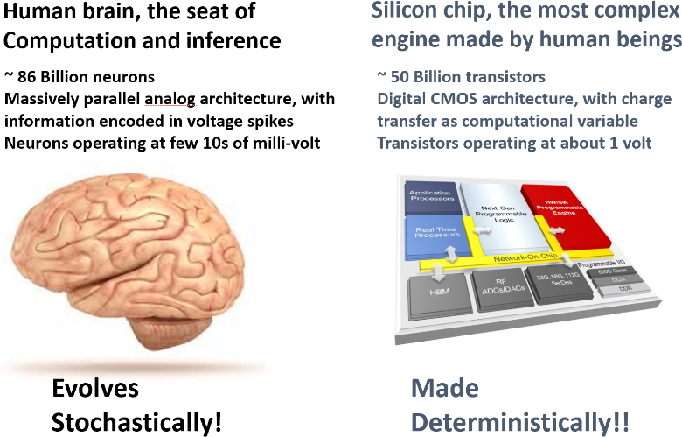
\includegraphics[scale=1.25]{src/Figures/chap1/chap1-fig06.jpg}
\caption{Contrast between neuronal and transistor circuits }\label{chap1-fig6}
\end{figure}

\centerline{\rule{10cm}{.5pt}}

\begin{figure}[H]
\centering
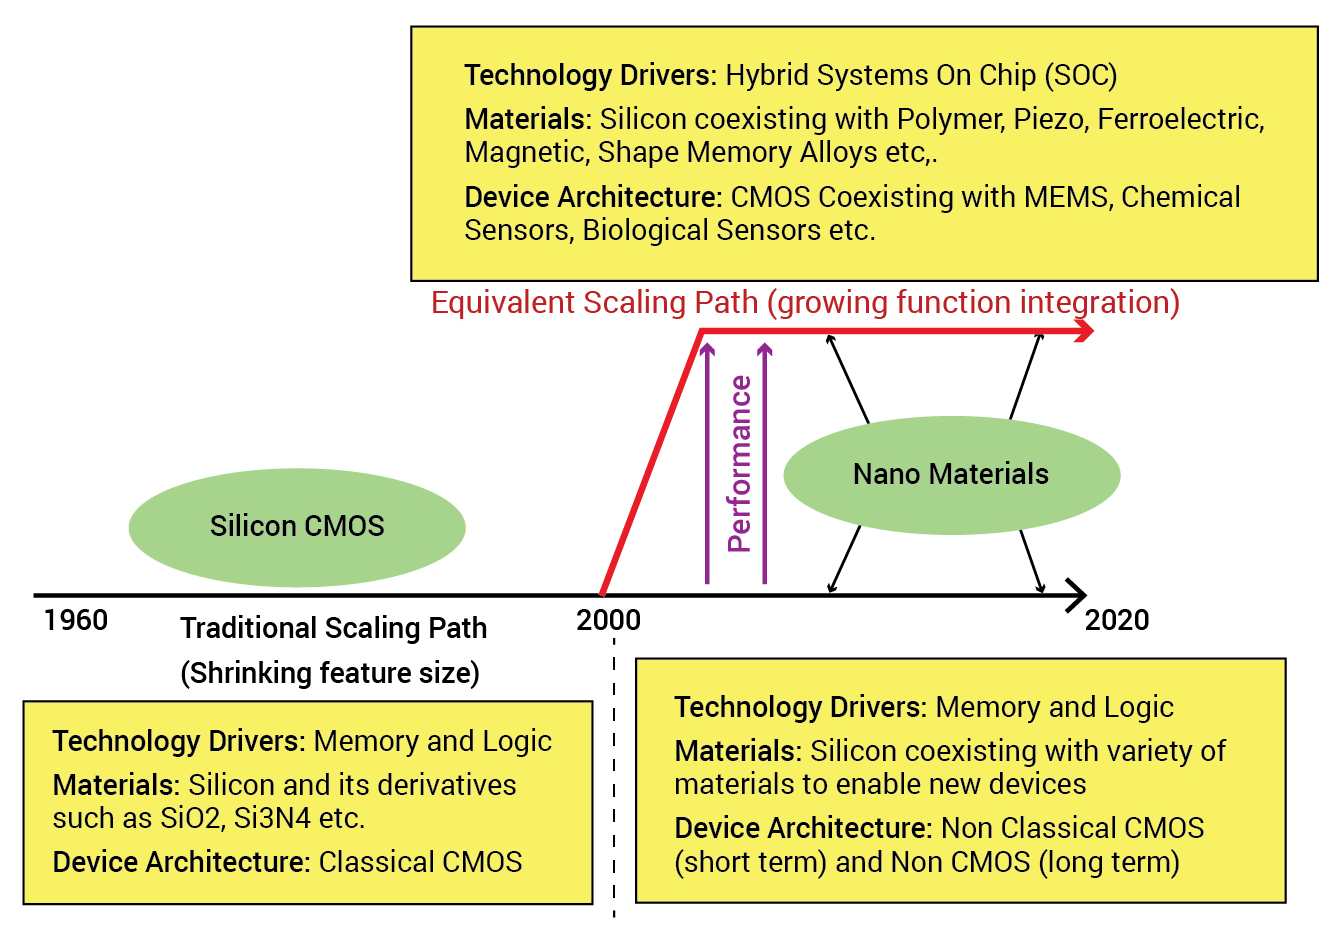
\includegraphics[scale=1.25]{src/Figures/chap1/chap1-fig07a.jpg}\qquad\qquad
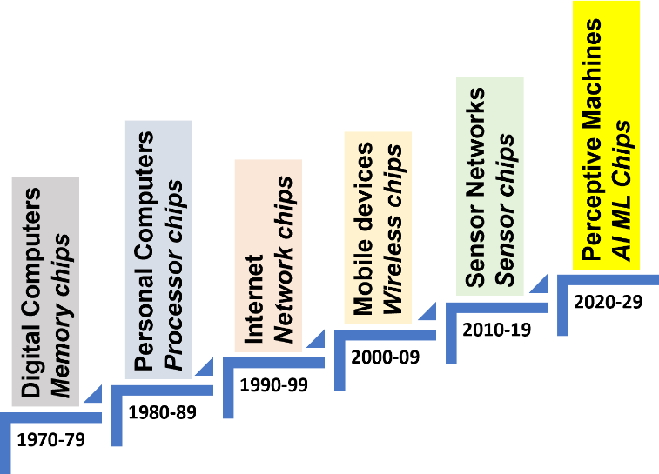
\includegraphics[scale=1.05]{src/Figures/chap1/chap1-fig07b.jpg}
\caption{The hybrid Systems on Chip through the integration of sensors and actuators with computation and storage engines. The emergence of new system drivers, results in the innovations in the chip technology.}\label{chap1-fig7}
\end{figure}

\vskip -1.25cm

\hfill\raisebox{-.1cm}{
\includegraphics[scale=.9]{src/Figures/circledC.eps}}


\begin{multicols}{2}
\begin{thebibliography}{99}
\bibitem{art1-key01} Nanotechnology Signature Initiative White Paper: Nanoelectronics for 2020 and Beyond 

\url{https://www.nano.gov/sites/default/files/pub_resource/nni_siginit_nanoelectronics_jul_2010.pdf}
\bibitem{art1-key02} Rainer Waser (Ed), Nanoelectronics and Information Technology: Advanced Electronic Materials and Novel Devices, 3rd Edition, Wiley-VCH, 2012
\bibitem{art1-key03} N.K. Upadhyay et. al., Emerging Memory Devices for Neuromorphic Computing”, Advanced Mateials Technology”, 2019 

\url{https://onlinelibrary.wiley.com/doi/epdf/10.1002/admt.201800589}
\bibitem{art1-key04} B Rajendran et. al., Low-Power Neuromorphic Hardware for Signal Processing Applications, 2019  \url{https://arxiv.org/pdf/1901.03690.pdf}
\bibitem{art1-key05} Girardin et. al. , Technologies and Sensors for the Internet of Things, Yole Development Report 

\url{http://www.yole.fr/iso_upload/Samples/Yole_IoT_June_2014_Sample.pdf}
\end{thebibliography}
\end{multicols}

\newpage
{\tabcolsep=10pt
\renewcommand{\arraystretch}{1.7}
\begin{longtable}{V{2.5}p{.95\textwidth}V{2.5}}
\clineB{1-1}{2.5}
\centerline{\large\bf Prof. Navakanta Bhat}\\[-.5cm]

\begin{wrapfigure}{l}{4.5cm}
\vspace{-10pt}

\includegraphics[scale=.07]{src/Figures/authors/NBhat.png}

\vspace{-5pt}
\end{wrapfigure}
Navakanta Bhat received his B.E. in Electronics and Communication from SJCE, University of Mysore in 1989, M.Tech. in Microelectronics from I.I.T. Bombay in 1992 and Ph.D. in Electrical Engineering from Stanford University, Stanford, CA in 1996. Then he worked at Motorola’s Networking and Computing Systems Group under Advanced Products R\&D Lab (APRDL)  in Austin, TX until 1999. At Motorola he worked on logic technology development and he was responsible for developing high performance transistor design and dual gate oxide technology for PowerPC microprocessors. He joined the Indian Institute of Science, Bangalore in 1999 where he is currently a Professor and Chair, Centre for Nano Science and Engineering. His current research is focused on Nanoelectronics device technology, Biosensors for point of care diagnostics and Gas sensors for pollution monitoring. He has 250 research publications in international journals and conferences and 10 granted US patents and 14 pending patents to his credit. He was instrumental in creating the National Nanofabrication Centre (NNfC) at IISc, Bangalore, benchmarked against the best university facilities in the world. He served as the chairman of NNfC administration committee (2010 – 2015).

\bigskip

He is an elected Fellow of the Indian National Academy of Engineering and elected Fellow of IEEE. He has received the Young Engineer Award (2003) from the Indian National Academy of Engineering, Swarnajayanti fellowship (2005) from the Department of Science and Technology, Govt. of India and Prof. Satish Dhavan award (2005) from the Govt. of Karnataka. He is also the recipient of IBM Faculty award 2007 and Outstanding Research Investigator award (2010) from DAE. For his translational research work, he has received Dr. Abdul Kalam Technology Innovation National Fellowship (2018), Prof. Rustum Choksi award for Excellence in Engineering Research (2017), Nina Saxena Technology Excellence award (2018), NASI Reliance Industries Platinum Jubilee award (2018) and BIRAC Innovator award (2018). He has also received the prestigious Infosys Prize (2018) for his contributions in Engineering and Computer Science category. 

\bigskip

He is currently (2016-2019) a member of the Board of Governors of the IEEE Electron Devices Society and also the Chair of Nanotechnology technical committee. He was the Editor of IEEE Transactions on Electron Devices, (2013-2015),  and the chief-editor of the IEEE TED special issue on “2D Materials for Electronic, Optoelectronic and Sensors”. He was the founding chair of the IEEE Electron Devices and Solid-State Circuits society, Bangalore chapter which was recognized as the Outstanding Chapter of the Year by the IEEE SSC society (2003) and IEEE EDS society (2005). He was the technical program chair for the International Conference on VLSI design and Embedded Systems (2007) and co-General chair of the International conference on Emerging Electronics (2012). He is a Distinguished Lecturer of the IEEE Electron Devices Society. 

\bigskip

He was the Chairman of the Human Resource Development and Infrastructure committee of the National Program on Micro and Smart Systems. He was the member of the committee set up by the Principal Scientific Advisor to Govt. of India to recommend strategies to develop semiconductor manufacturing ecosystem in India.  

\bigskip

He is the founder and promoter of a startup company, PathShodh Healthcare Pvt Ltd (\url{www.pathshodh.com}).   Based on his group’s research in biosensors, PathShodh has developed the first of its kind multi-analyte point-of-care diagnostic device for 5 blood tests and 3 urine tests, related to multiple chronic diseases including diabetes and its complications, anemia and malnutrition, kidney and liver diseases. For this technology, PathShodh has received multiple recognitions : Confederation of Indian Industry (CII) Industrial Innovation Award 2017, for the most promising start-up and CII Grand Jury Award for Innovation, 2017; Federation of Indian Chambers of Commerce and Industry (FICCI) Healthcare Excellence award, 2017 for the best start-up of the year; Design Impact award for Social change by Titan. \\
\clineB{1-1}{2.5}
\end{longtable}}\relax
